\section{Objectives}
Rebuild the DC characterization experiments for NMOS and PMOS according to Lab 1 of the supplied \textit{DIC Lab.pdf} (PDF pages 3--9), covering all four experimental steps and four discussion questions. The objectives are diode-connected transfer curves, output curves at different gate biases, channel-length dependence of output slope, and semilog analysis of weak-inversion behavior.

This is a teaching adaptation using a model library supplied separately by the user. The handout uses an older process with biases reaching 2.5--4 V. The present terminal-voltage magnitudes are limited to 1.0 V for comparison while retaining the baseline handout dimensions. The selected 1.0 V is a simulation condition, not a verified rating of the encrypted model. These results do not reproduce the original process values or breakdown region.

\section{Spec mapping}
The handout steps and questions define the checks below. ``Simulated'' means successful execution under the stated adapted conditions; it does not mean that the original process values have been reproduced.
\begin{center}
\setlength{\tabcolsep}{3pt}
\begin{tabular}{p{0.42\linewidth}p{0.29\linewidth}p{0.23\linewidth}}
\toprule
Requirement (PDF page) & Implementation & Check \\
\midrule
Step 1: diode-connected transfer (8) & \texttt{01\_diode\_n/p.sp} & Simulated; adapted bias \\
Step 2: separate G/D; gate sweep (8) & \texttt{02\_output\_n/p.sp} & Simulated; adapted range \\
Step 3: fixed W; vary L (8) & \texttt{03\_length.sp} & Simulated; adapted bias \\
Step 4: semilog weak-inversion curve (8) & \texttt{04\_subthreshold.sp} & Fitted; limited interval \\
Question 1: increasing W/L (9) & \texttt{01\_diode\_n/p.sp} & Three widths compared \\
Question 2: equal-geometry N/P ratio (9) & \texttt{05\_equal\_geometry.sp} & Current, not mobility \\
Question 3: output slope versus L (9) & \texttt{03\_length.sp} & Secant slopes measured \\
Question 4: weak-inversion slope (9) & \texttt{04\_subthreshold.sp} & Approximate slopes fitted \\
\bottomrule
\end{tabular}
\end{center}

\section{Circuit and design derivation}
Step 1 shorts Gate to Drain as shown in Fig. 1.2(a), instead of sweeping $V_{GS}$ with a fixed $V_{DS}$. This corrects a material mismatch in the reference source files. Only Step 2 separates Gate and Drain and drives them independently. NMOS Source/Bulk are grounded. PMOS Source/Bulk are also grounded, with negative Gate/Drain voltages, allowing direct comparison of $V_{SG}$ and $V_{SD}$ magnitudes.

The baseline dimensions are $W_n=0.6\,\mu\mathrm m$, $W_p=1.8\,\mu\mathrm m$, and $L=0.25\,\mu\mathrm m$. The model names are \texttt{nmos/pmos}; channel lengths are not indiscriminately reduced to 90 nm. All MOS instances explicitly specify \texttt{W=} and \texttt{L=}, and decreasing PMOS sweeps use negative increments.

A long-channel approximation is
\[
 I_D\simeq\frac{\mu C_{ox}}{2}\frac WL(V_{GS}-V_T)^2(1+\lambda V_{DS}).
\]
Increasing W generally increases current. Reducing L changes both $W/L$ and potentially short-channel effects. This equation explains trends; numerical values come from the supplied model. Output slope is evaluated as the secant over 0.8--1.0 V,
\[
g_{ds,\mathrm{sec}}=\frac{|I_D(1.0)|-|I_D(0.8)|}{0.2},
\]
which is not itself $\lambda$. For the semilog region,
\[
S=\left(\frac{d\log_{10}|I_D|}{d|V_{GS}|}\right)^{-1},
\]
in V/dec. A larger S means a smaller current slope on the semilog plot.

\section{Simulation setup}
PrimeSim HSPICE S-2021.09 win64 was used at 25\,$^\circ$C. Public decks mark the model setup location; private execution copies load the separately supplied library. The seven independent \texttt{.sp} files can be opened separately in the simulator; \texttt{.alter} defines parameter comparisons. Outputs include \texttt{.sw*} waveforms, \texttt{.ms*} measurements and printed data in \texttt{.lis}.

\begin{itemize}
\item Diode connection: $|V_{GS}|=|V_{DS}|=0$--1 V in 1 mV steps; W is 1, 2 or 4 times its baseline value.
\item Output curves: $|V_{DS}|=0$--1 V in 1 mV steps; $|V_{GS}|=0,0.2,0.4,0.6,0.8,1.0$ V.
\item Length comparison: $L=0.25,0.50,0.75,1.00\,\mu\mathrm m$, fixed W, and $|V_{GS}|=0.6$ V for both polarities. This differs from the handout's 1.6 V NMOS / 0.9 V PMOS biases, so only the analogous trend under the adapted conditions is checked.
\item Weak-inversion curves: $|V_{GS}|=0$--0.5 V; $|V_{DS}|=1.0,0.6,0.3$ V. The fit uses only 0.15--0.25 V; the full sweep is not labelled weak inversion.
\item Equal-geometry comparison: both devices use $W/L=0.6/0.25\,\mu\mathrm m$, $|V_{DS}|=0.8$ V, and the current ratio is measured at $|V_{GS}|=0.8$ V.
\end{itemize}
\texttt{.measure} extracts selected numerical features from a waveform; it does not replace the complete curve. Figures are redrawn from this run's printed HSPICE data through CSV files in \texttt{validation/dic\_pilot/}. Voltage-source current has the opposite sign to device Drain current; tabulated currents are magnitudes.

HSPICE also reports suppressed warnings associated with encrypted blocks. A diagnostic run with \texttt{WARNLIMIT=100} reveals no further detail. Its measurements agree with the original run, but this does not establish that the warnings are harmless; a warning-free simulation is not claimed.

\section{Results and specification checks}
All analyses of the seven decks concluded normally, without \texttt{**error**} or failed measurements. Actual diode-connected currents at $|V_{GS}|=1.0$ V are:
\begin{center}
\setlength{\tabcolsep}{3pt}
\begin{tabular}{lrr}
\toprule
W multiplier & $|I_{Dn}|$ ($\mu$A) & $|I_{Dp}|$ ($\mu$A) \\
\midrule
1 & 198.491 & 112.529 \\
2 & 399.898 & 225.674 \\
4 & 802.707 & 451.963 \\
\bottomrule
\end{tabular}
\end{center}

The current is approximately proportional to W, but the ratios are not exact integers. With equal geometry and $|V_{GS}|=|V_{DS}|=0.8$ V, NMOS current is 111.7734\,$\mu$A, PMOS current is 20.4637\,$\mu$A, and their magnitude ratio is 0.183082.
\begin{figure}[htbp]
\centering
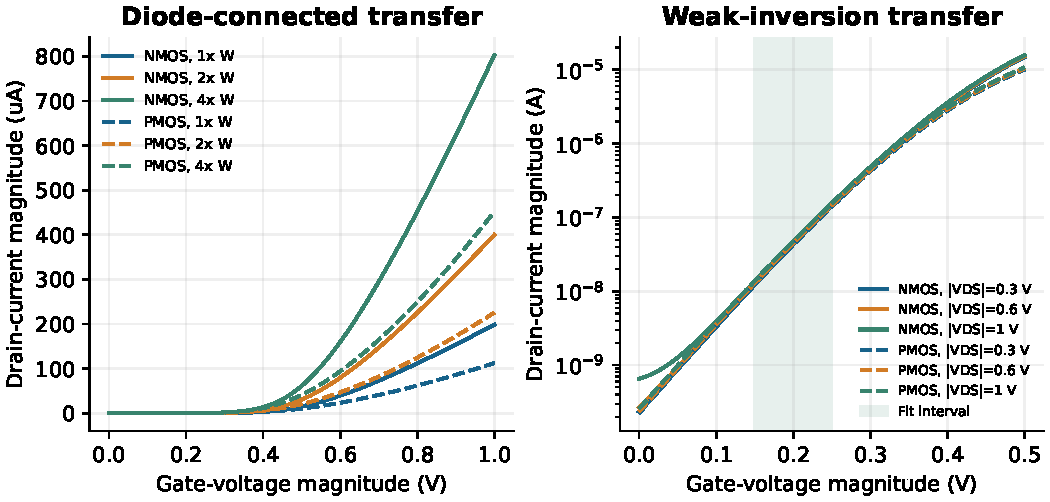
\includegraphics[width=\linewidth]{figures/dic01_characteristics.pdf}
\caption{Diode-connected and semilog transfer curves redrawn from the actual HSPICE results, not WaveView screenshots. The weak-inversion fit uses only the interval specified in the text.}
\end{figure}
\begin{figure}[htbp]
\centering
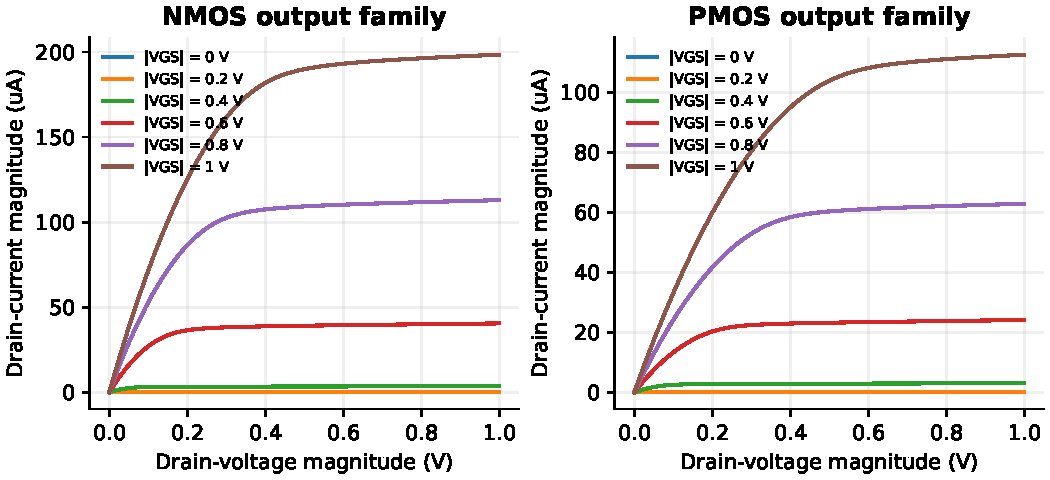
\includegraphics[width=\linewidth]{figures/dic01_output.pdf}
\caption{NMOS and PMOS output-characteristic families redrawn from actual HSPICE data. Each curve uses a fixed gate bias; drain-voltage and current magnitudes are compared.}
\end{figure}

With $|V_{GS}|=0.6$ V, the following output secant slopes over 0.8--1.0 V decrease with L for both polarities.
\begin{center}
\setlength{\tabcolsep}{3pt}
\begin{tabular}{lrr}
\toprule
$L$ ($\mu$m) & $g_{ds,n}$ ($\mu$S) & $g_{ds,p}$ ($\mu$S) \\
\midrule
0.25 & 2.4410 & 1.6097 \\
0.50 & 0.6447 & 0.3574 \\
0.75 & 0.3445 & 0.1795 \\
1.00 & 0.2261 & 0.1141 \\
\bottomrule
\end{tabular}
\end{center}
\begin{figure}[htbp]
\centering
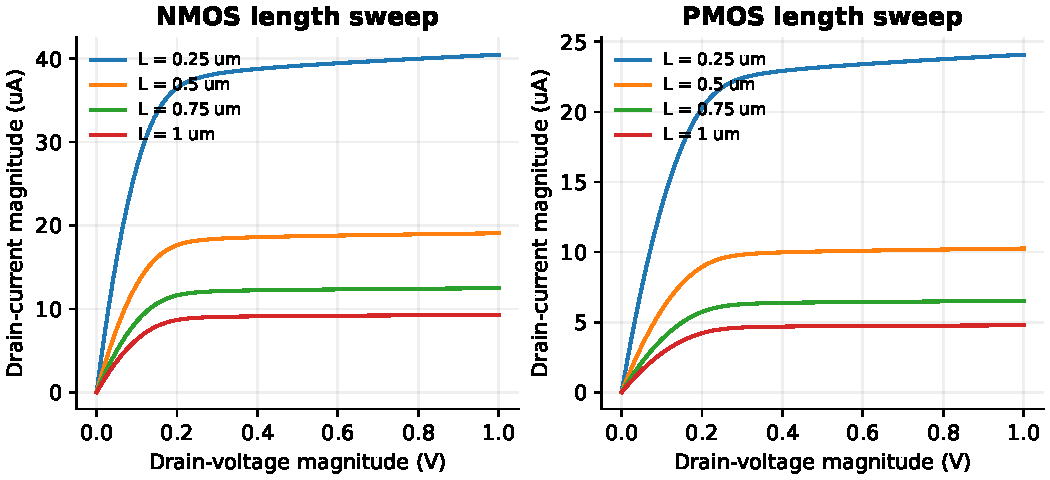
\includegraphics[width=\linewidth]{figures/dic01_length.pdf}
\caption{NMOS and PMOS length comparisons redrawn from actual HSPICE data, with fixed widths and gate biases. Each curve identifies its channel length.}
\end{figure}

Semilog fits over 0.15--0.25 V give:
\begin{center}
\setlength{\tabcolsep}{3pt}
\begin{tabular}{lrrrr}
\toprule
$|V_{DS}|$ (V) & $S_n$ (mV/dec) & $S_p$ (mV/dec) & $R_n^2$ & $R_p^2$ \\
\midrule
1.0 & 94.09 & 95.33 & 0.999865 & 0.999784 \\
0.6 & 93.65 & 95.13 & 0.999837 & 0.999789 \\
0.3 & 93.55 & 94.99 & 0.999837 & 0.999793 \\
\bottomrule
\end{tabular}
\end{center}

At $|V_{DS}|=1$ V, local S spans approximately 91.06--99.11 mV/dec for NMOS and 90.44--101.00 mV/dec for PMOS. The high $R^2$ supports an approximately exponential current relation in this interval. Model $V_T$ or region indicators were not independently extracted, so this is described as an approximate weak-inversion fit, not a model-internal confirmation that every point is below threshold.

\section{Discussion}
\textbf{Question 1:} Increasing W at fixed L gives an approximately proportional current increase, consistent with the first-order $W/L$ expression. Changing L cannot be predicted by the same scaling alone because effective length, parasitics and short-channel behavior may also change.

\textbf{Question 2:} Equal W/L does not guarantee $|I_{Dp}|/I_{Dn}=\mu_p/\mu_n$. Even a square-law derivation additionally requires matched overdrive and other parameters. Threshold voltage, mobility degradation and velocity saturation in the supplied model can affect the currents. The measured 0.183082 is a current ratio at the stated bias, not an extracted mobility ratio of the encrypted model.

\textbf{Question 3:} As L increases from 0.25 to 1.00\,$\mu$m, both output slopes decrease, indicating reduced sensitivity to Drain voltage. This agrees qualitatively with channel-length modulation, but $\lambda$ was not extracted from a single secant slope.

\textbf{Question 4:} Using $|V_{GS}|$ as the horizontal axis, the PMOS fit at 1 V Drain magnitude has a slightly larger S, hence a slightly smaller semilog current slope. Local S changes with Gate bias, and the N/P ranges overlap. This is not a universal ranking across biases or processes. Differences depend on capacitive coupling, subthreshold factors and model parameters; the encrypted model does not expose independently verified parameter values in this work.

\section{Conclusion}
All four experimental steps and four questions have corresponding code, actual HSPICE data and discussion. The rewrite corrects the missing diode connection and the PMOS sweep direction in the reference code. Results support increasing current with width, decreasing output slope with length, and approximately exponential conduction within the selected fitting interval. Checks apply to the stated adapted conditions; original-process high-voltage curves, breakdown behavior and internal model threshold indicators remain outside the verified results.
